\documentclass[12pt,a4paper]{article}

\usepackage[a4paper,top=3.1cm,bottom=3.0cm,left=2.5cm,right=2.0cm,headheight=16pt]{geometry}
\usepackage[T1]{fontenc}
\usepackage[utf8]{inputenc}
\usepackage{newtxtext}
\usepackage{newtxmath}
\usepackage{amsmath}
\usepackage{array}
\usepackage{multirow}
\usepackage{graphicx}
\usepackage{tikz}
\usepackage{pgfplots}
\usepackage{caption}
\usepackage{fancyhdr}
\usepackage{indentfirst}
\usepackage{microtype}
\usepackage[hidelinks]{hyperref}
\usepackage{cite}
\usepackage{url}
\usepackage{siunitx}
\usepackage{xcolor}

\pgfplotsset{compat=1.18}
\usetikzlibrary{arrows.meta,positioning,fit,calc,shapes.geometric,matrix}

\setlength{\parindent}{1.25cm}
\setlength{\parskip}{0pt}
\emergencystretch=2em
\raggedbottom

\renewcommand{\figurename}{Fig.}
\captionsetup[figure]{font=small,justification=centering,labelsep=period}

\newcommand{\shorttitle}{Cloud Email Analyzer}
\newcommand{\conferenceheader}{Sesiunea de Comunicări Științifice Studențești, SCCS 2026, Secțiunea TODO: 12.X}

\pagestyle{fancy}
\fancyhf{}
\fancyhead[L]{\small \shorttitle}
\fancyhead[R]{\small \thepage}
\renewcommand{\headrulewidth}{0.4pt}

\fancypagestyle{firstpage}{
  \fancyhf{}
  \fancyhead[C]{\small \conferenceheader}
  \renewcommand{\headrulewidth}{0.4pt}
}

\makeatletter
\renewcommand\section{\@startsection {section}{1}{\z@}%
  {-2.2ex \@plus -1ex \@minus -.2ex}%
  {1.1ex \@plus .2ex}%
  {\centering\normalfont\normalsize\bfseries}}
\renewcommand\subsection{\@startsection{subsection}{2}{\z@}%
  {-1.6ex\@plus -0.8ex \@minus -.2ex}%
  {0.8ex \@plus .2ex}%
  {\normalfont\normalsize\bfseries}}
\renewcommand\subsubsection{\@startsection{subsubsection}{3}{\z@}%
  {-1.2ex\@plus -0.6ex \@minus -.2ex}%
  {0.6ex \@plus .2ex}%
  {\normalfont\normalsize\itshape}}
\makeatother

\newenvironment{templateabstract}[1]{%
  \begin{center}
  \begin{minipage}{0.86\textwidth}
  \small\itshape\noindent\textbf{#1:}\ %
}{%
  \end{minipage}
  \end{center}
}

\newcommand{\keywordline}[2]{%
  \begin{center}
  \begin{minipage}{0.86\textwidth}
  \small\noindent\textbf{#1:} #2
  \end{minipage}
  \end{center}
}

\newcommand{\papertablecaption}[2]{%
  \refstepcounter{table}\label{#1}%
  \begin{flushright}\small\itshape Table~\thetable\end{flushright}%
  \vspace{-1.0em}%
  \begin{center}\small\bfseries #2\end{center}%
  \vspace{-0.75em}%
}

\renewcommand{\refname}{\centering\normalfont\normalsize\bfseries R E F E R E N C E S}

\begin{document}
\thispagestyle{firstpage}

\begin{center}
{\bfseries\large\MakeUppercase{Cloud Email Analyzer: An Event-Driven Architecture for Email Threat Triage with ML-Assisted Classification and Attachment Scanning}}\par
\vspace{1.0em}
{\normalsize Authors -- TODO: First AUTHOR$^{1}$, TODO: Second AUTHOR$^{2}$}\par
\vspace{0.3em}
{\normalsize Scientific Coordinator -- TODO: Academic title and full name$^{3}$}\par
\end{center}

\vspace{1.0em}

\begin{templateabstract}{Abstract}
Cloud Email Analyzer is an AWS-oriented email security platform for cloud-native message triage. The system receives inbound mail with SES for domains whose MX records are managed in Route53, preserves raw MIME objects in S3, normalizes processing through a canonical \texttt{MailReceived} event, routes events with EventBridge, orchestrates Lambda stages with Step Functions, applies TF-IDF-based phishing classification, scans attachments with ClamAV, stores ledger state and artifact pointers in DynamoDB, and exposes verdicts through an authenticated review dashboard.
\end{templateabstract}

\keywordline{Keywords}{email security, AWS, event-driven architecture, serverless workflow, phishing classification, attachment scanning, DynamoDB}

\begin{templateabstract}{Rezumat}
Cloud Email Analyzer este o platformă de securitate e-mail orientată spre AWS, destinată triajului mesajelor suspecte. Sistemul primește mesaje prin SES pentru domenii cu înregistrări MX gestionate în Route53, păstrează obiectele MIME brute în S3, normalizează procesarea prin evenimentul \texttt{MailReceived}, rutează evenimentele cu EventBridge, orchestrează etapele Lambda prin Step Functions, clasifică phishing-ul prin TF-IDF, scanează atașamentele cu ClamAV, stochează starea în DynamoDB și afișează verdictele într-un tablou de bord autentificat.
\end{templateabstract}

\keywordline{Cuvinte cheie}{securitate e-mail, AWS, arhitectură orientată pe evenimente, workflow serverless, clasificare phishing, scanare atașamente, DynamoDB}

\vfill
\noindent{\small
$^{1}$ TODO: Student, group TODO, Faculty TODO, e-mail: TODO.\\
$^{2}$ TODO: Student, group TODO, Faculty TODO, e-mail: TODO.\\
$^{3}$ TODO: Scientific coordinator affiliation, department, e-mail: TODO.}
\vspace{1.0em}
\newpage

\section{Introduction}

Email security systems have to treat an inbound message as more than a visible subject line and body. The raw message may contain MIME parts, alternative HTML and plain-text bodies, envelope recipients that differ from the displayed headers, embedded URLs, file attachments, authentication hints, and security verdicts produced by other systems. A useful analysis platform must therefore preserve the original message while extracting evidence into a form that can be queried, audited, and reviewed by users with different privileges.

Cloud Email Analyzer addresses this operational problem through a staged, event-driven AWS architecture. The system receives raw email with Amazon SES for domains whose MX records are managed in Route53, stores the MIME source in S3, parses headers and bodies, extracts attachments, runs a phishing classifier on message text, scans files with ClamAV, persists a review ledger in DynamoDB, and presents the result in a FastAPI and React dashboard. LocalStack is used during development to exercise AWS-shaped service boundaries without changing the cloud design; it is an engineering aid, not the architectural endpoint.

The central design decision is the canonical \texttt{MailReceived} event. After inbound mail is accepted and the MIME object is stored, later stages operate on an event containing tenant, message, envelope, header, verdict, and storage-pointer metadata. That boundary prevents MIME analysis, detector execution, and dashboard review from depending directly on the mechanics of SMTP receipt. It also gives the system a stable audit point: every derived artifact, detector output, and user-visible verdict can be traced back to the same message identifier.

The contribution of the project is an integrated email-triage workflow rather than a new detector in isolation. The phishing classifier is a practical supervised text model, and the attachment scanner uses an established antivirus engine. The project value lies in connecting these pieces with deterministic storage, staged orchestration, authorization, administrator review, and audit logging so that an inbound message becomes reviewable security evidence.

The remainder of the paper is organized as follows. Section 2 positions the project against related work. Section 3 summarizes the system goals and requirements. Section 4 presents the event-driven AWS architecture and the canonical event. Section 5 details the processing pipeline and persistent data model. Section 6 describes the classifier, attachment scanner, and final-verdict rules. Section 7 explains the user and administrator dashboard. Section 8 reports evaluation results from the ML artifacts and implementation checks. Section 9 states limitations and future work. Section 10 concludes the paper.

\section{Related Work and Positioning}

Machine-learning-based phishing email detection has a long research history. Fette, Sadeh, and Tomasic introduced PILFER, a supervised detector based on deception-oriented features, and reported high phishing detection with very low legitimate-mail misclassification on their evaluation set \cite{fette2007learning}. Later surveys explain why the problem is still not solved by a single classifier: phishing email filtering combines URL, header, content, reputation, and machine-learning signals, while adaptation and evasion remain persistent difficulties \cite{almomani2013survey,khonji2013survey}. Recent comparative work continues this detector-centric direction by evaluating TF-IDF, Word2Vec, BERT, and traditional classifiers for phishing email classification \cite{altawil2024comparative}.

Cloud Email Analyzer uses that line of work as one layer rather than as the whole system. Its classifier is a TF-IDF-based supervised model, appropriate for efficient text scoring inside a workflow. The architectural question is different from the one answered by detector-only papers: after a detector produces a score, the platform still has to preserve the raw message, store derived artifacts, scan attachments, aggregate heterogeneous verdicts, enforce user-specific access, and keep an audit trail.

D-Fence is closer to this project because it presents a multi-module phishing email detection system that combines structure, text, and URL analysis for enterprise-scale phishing detection \cite{lee2021dfence}. Cloud Email Analyzer takes a complementary route. Instead of optimizing a new detector ensemble, it emphasizes cloud ingestion, persistent evidence, review ergonomics, and operational traceability around detector outputs. The comparison is useful because it separates two dimensions of email security work: how accurately a detector recognizes malicious intent, and how the surrounding platform turns detector evidence into controlled review and response.

Attachment handling introduces a second research thread. Rudd, Harang, and Saxe study malicious email attachment detection across heterogeneous file types and show that attachment-focused ML can be treated as a separate detection problem \cite{rudd2018meade}. Zhang et al. show that MIME parsing ambiguity can let adversaries evade email attachment detectors, strengthening the case for preserving the raw message and separating MIME parsing from later detector outputs \cite{zhang2024inbox}. Cloud Email Analyzer follows this separation: the parser extracts evidence and file artifacts, the scanner evaluates each attachment, and the dashboard exposes per-file scan state instead of collapsing all file evidence into an opaque message label.

The workflow layer is related to serverless computing research. Serverless systems are commonly decomposed into small stateless functions that communicate through storage and cloud services, while workflow orchestration coordinates longer application logic \cite{marin2022serverless}. Triggerflow and related work discuss state machines, DAGs, and trigger-based orchestration as patterns for composing event-driven functions \cite{garcia2021triggerflow}. Cloud Email Analyzer applies this pattern to email security: SES and Route53 provide ingress, EventBridge carries the normalized event, Step Functions coordinates analysis stages, S3 stores large artifacts, and DynamoDB stores queryable state.

\begin{table}[!htbp]
\papertablecaption{tab:related}{Positioning against selected related work}
\centering
\footnotesize
\begin{tabular}{|>{\raggedright\arraybackslash}p{0.24\textwidth}|>{\raggedright\arraybackslash}p{0.34\textwidth}|>{\raggedright\arraybackslash}p{0.32\textwidth}|}
\hline
\textbf{Research line} & \textbf{Main emphasis in related work} & \textbf{Cloud Email Analyzer emphasis} \\
\hline
Phishing ML detectors & Supervised classification of phishing messages using engineered, text, URL, or embedding features. & Uses a TF-IDF classifier as one detector inside a larger triage workflow. \\
\hline
Multi-module phishing systems & Combines several email components to improve phishing detection and reduce single-signal blind spots. & Combines text verdicts with attachment scanning, storage, authorization, and audit review. \\
\hline
Attachment and MIME research & Studies malicious attachments and evasion through parsing ambiguity. & Preserves raw MIME, stores parsed artifacts, and exposes per-attachment scan evidence. \\
\hline
Serverless workflow research & Coordinates event-driven functions through state machines, triggers, and cloud services. & Applies event-driven orchestration to email ingestion, analysis, verdict aggregation, and review. \\
\hline
\end{tabular}
\end{table}


\section{System Overview and Requirements}

Cloud Email Analyzer is designed as an AWS email security inbox for organizations that need to inspect suspicious messages without losing the original evidence. The product flow is direct: receive an email, store the raw MIME object, extract structured evidence, run detectors, compute verdicts, and expose the result to the appropriate user or administrator. The reviewer should see both the short verdict and the supporting evidence: sender and recipients, subject, parsed text and HTML, URLs and domains, attachment metadata, hashes, scan signatures, classifier confidence, processing timeline, and audit trail.

The AWS ingress layer uses Route53-hosted DNS/MX records and Amazon SES receipt rules. SES can receive mail for a verified domain and store accepted messages in S3 \cite{aws_ses_receiving}. An ingestion adapter then publishes the canonical \texttt{MailReceived} event, after which the rest of the system is independent of SMTP details. This choice also supports development with LocalStack: the team can exercise S3, EventBridge, Step Functions, Lambda-style handlers, and DynamoDB during implementation while keeping the same event shape and storage boundaries used by the AWS design.

The system requirements can be grouped into six categories. First, raw-message preservation is required because later stages and reviewers may need to inspect or reprocess the original MIME object. Second, ingestion must be normalized so the analysis pipeline receives a stable event contract. Third, processing must be staged because recipient mapping, MIME parsing, ML classification, file scanning, and aggregation have different failure modes and outputs. Fourth, the database model must support both user inbox queries and security-administrator review. Fifth, backend authorization must be authoritative because hiding navigation elements in the frontend is not a security control. Sixth, review must be auditable: security-relevant actions such as login, message view, reprocess, and attachment download should leave records.

\begin{table}[!htbp]
\papertablecaption{tab:components}{Cloud Email Analyzer components and responsibilities}
\centering
\small
\begin{tabular}{|>{\raggedright\arraybackslash}p{0.22\textwidth}|>{\raggedright\arraybackslash}p{0.43\textwidth}|>{\raggedright\arraybackslash}p{0.25\textwidth}|}
\hline
\textbf{Component} & \textbf{Responsibility} & \textbf{Main output} \\
\hline
SES and Route53 ingress & Receive mail with SES for a domain whose MX records are managed in Route53, then place the raw MIME object in cloud storage. & Raw message object and envelope metadata. \\
\hline
EventBridge boundary & Carry the canonical \texttt{MailReceived} event into the analysis workflow. & Stable event contract. \\
\hline
Step Functions workflow & Orchestrate the sequential stages with retry behavior. & Ordered processing state. \\
\hline
Ledger and recipient stages & Create the message row, map envelope recipients to owners, and write inbox rows. & Message ownership and inbox visibility. \\
\hline
Parser stage & Parse MIME headers, text, HTML, and attachments; store parsed JSON and file artifacts. & Parsed body artifact and attachment records. \\
\hline
Detection stages & Run packaged TF-IDF classifier inference and ClamAV attachment scanning. & ML verdicts and per-file scan evidence. \\
\hline
Aggregation stage & Combine ML and attachment evidence into message and inbox verdicts. & Final verdict: \texttt{SAFE}, \texttt{SUSPICIOUS}, or \texttt{UNSAFE}. \\
\hline
FastAPI API and React dashboard & FastAPI enforces authorization and exposes message/admin endpoints; React presents the user and administrator review workflows. & Authenticated user/admin security inbox. \\
\hline
\end{tabular}
\end{table}


Table~\ref{tab:components} summarizes the main components. The design is intentionally practical: small services perform bounded tasks, object storage carries large artifacts, and DynamoDB tables store queryable state for the API and dashboard. This division keeps the system understandable for presentation while preserving the vocabulary of production event-driven systems.

\section{Event-Driven AWS Architecture}

The architecture centers on a normalized event boundary. Amazon SES receives inbound mail for a domain whose MX records are managed in Route53 and stores the raw MIME message in S3. An ingestion adapter publishes a \texttt{MailReceived} event that contains the message identifier, tenant, received timestamp, raw object pointer, envelope sender, envelope recipients, header hints, and SES verdict metadata. The event carries metadata and pointers; it does not carry raw email bodies, HTML, or attachment bytes.

\begin{figure}[!htbp]
\centering
\resizebox{\textwidth}{!}{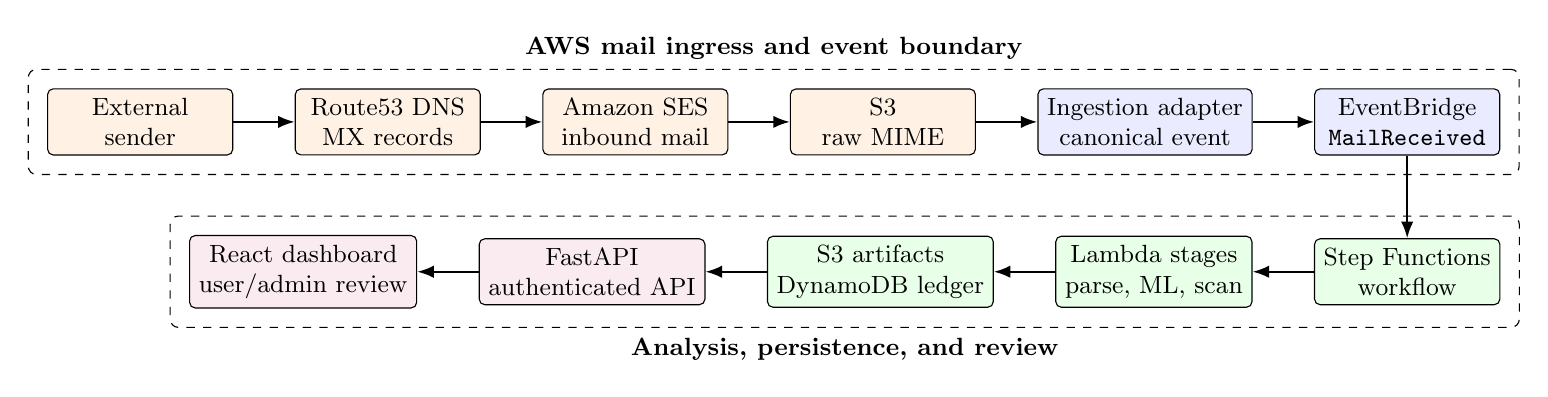
\begin{tikzpicture}[
  font=\small,
  node distance=0.72cm and 0.78cm,
  box/.style={draw, rounded corners=2pt, align=center, minimum width=2.35cm, minimum height=0.78cm, fill=gray!7},
  ingress/.style={box, fill=orange!10},
  event/.style={box, fill=blue!8},
  process/.style={box, fill=green!9},
  review/.style={box, fill=purple!8},
  arrow/.style={-{Latex[length=2.1mm]}, thick}
]
\node[ingress] (sender) {External\\sender};
\node[ingress, right=of sender] (route53) {Route53 DNS\\MX records};
\node[ingress, right=of route53] (ses) {Amazon SES\\inbound mail};
\node[ingress, right=of ses] (raw) {S3\\raw MIME};
\node[event, right=of raw] (publisher) {Ingestion adapter\\canonical event};
\node[event, right=of publisher] (bus) {EventBridge\\\texttt{MailReceived}};

\node[process, below=1.05cm of bus] (sfn) {Step Functions\\workflow};
\node[process, left=of sfn] (lambda) {Lambda stages\\parse, ML, scan};
\node[process, left=of lambda] (stores) {S3 artifacts\\DynamoDB ledger};
\node[review, left=of stores] (api) {FastAPI\\authenticated API};
\node[review, left=of api] (ui) {React dashboard\\user/admin review};

\draw[arrow] (sender) -- (route53);
\draw[arrow] (route53) -- (ses);
\draw[arrow] (ses) -- (raw);
\draw[arrow] (raw) -- (publisher);
\draw[arrow] (publisher) -- (bus);
\draw[arrow] (bus) -- (sfn);
\draw[arrow] (sfn) -- (lambda);
\draw[arrow] (lambda) -- (stores);
\draw[arrow] (stores) -- (api);
\draw[arrow] (api) -- (ui);

\node[draw, dashed, rounded corners=3pt, fit=(sender)(route53)(ses)(raw)(publisher)(bus), inner sep=0.24cm, label={[font=\small\bfseries]above:AWS mail ingress and event boundary}] {};
\node[draw, dashed, rounded corners=3pt, fit=(sfn)(lambda)(stores)(api)(ui), inner sep=0.24cm, label={[font=\small\bfseries]below:Analysis, persistence, and review}] {};
\end{tikzpicture}
}
\caption{AWS-oriented architecture of Cloud Email Analyzer from inbound mail to authenticated review.}
\label{fig:architecture}
\end{figure}

Figure~\ref{fig:architecture} shows the end-to-end cloud shape. EventBridge is used because event buses route events from sources to targets and rules evaluate event patterns before delivery \cite{aws_eventbridge_bus}. Step Functions supplies the workflow layer; AWS describes a state machine as a workflow composed of event-driven steps, with task states representing units of work performed by AWS services or APIs \cite{aws_step_functions}. S3 keeps large immutable artifacts, and DynamoDB keeps compact queryable state.

The canonical event follows EventBridge conventions with a source, a detail type, and a detail object. The detail contains identity, envelope, header, storage, and upstream-verdict metadata. The important architectural point is that later pipeline stages depend on the event contract, not on the exact mail-receipt mechanism. This keeps ingestion, processing, and review loosely coupled.

The repository also defines deterministic identifiers. A stable message identifier can be derived from the SHA-256 digest of raw message bytes. Attachment identifiers combine an index, a SHA-256 prefix, and a sanitized filename. These identifiers are not proofs of safety, but they make artifact pointers and database rows predictable across repeated processing. That property matters for idempotency: duplicate event handling should update the same logical message rather than creating unrelated records.

LocalStack is part of the development workflow because it lets the team run AWS-shaped services locally while validating the same boundaries: object storage, event routing, workflow orchestration, Lambda-style execution, and DynamoDB state. The paper keeps that detail in the engineering background. The system being documented is the AWS-oriented architecture in Fig.~\ref{fig:architecture}.

\section{Processing Pipeline and Data Model}

The Step Functions workflow is sequential in the current design:

\begin{equation}
\begin{aligned}
\texttt{MailReceived} &\rightarrow \texttt{InitLedger}
\rightarrow \texttt{ResolveRecipients}
\rightarrow \texttt{ParseEmail} \\
&\rightarrow \texttt{PhishingML}
\rightarrow \texttt{AttachmentScan}
\rightarrow \texttt{AggregateVerdicts}.
\end{aligned}
\label{eq:pipeline}
\end{equation}

Each task includes retry behavior, and the stages are written so repeated invocations update deterministic records rather than creating a new logical message each time. The design could later parallelize ML and attachment scanning because both depend on parsed artifacts, not on each other. The sequential flow is easier to observe, explain, and audit.

\begin{figure}[!htbp]
\centering
\resizebox{\textwidth}{!}{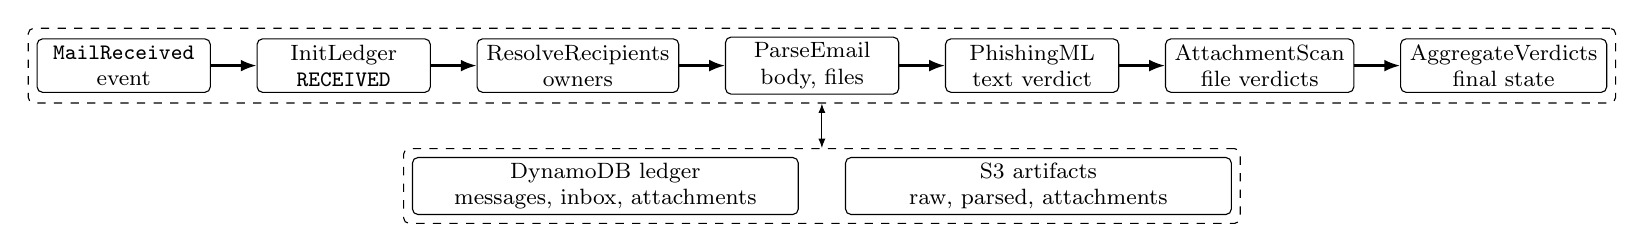
\begin{tikzpicture}[
  font=\footnotesize,
  stage/.style={draw, rounded corners=2pt, align=center, minimum width=2.2cm, minimum height=0.68cm, inner ysep=2pt, fill=white},
  store/.style={draw, rounded corners=2pt, align=center, minimum width=4.9cm, minimum height=0.54cm, inner ysep=2pt, fill=white},
  arrow/.style={-{Latex[length=2mm]}, thick},
  groupbox/.style={draw, dashed, rounded corners=2pt, inner sep=3pt},
  groupconn/.style={{Latex[length=1.2mm]}-{Latex[length=1.2mm]}, thin},
  node distance=0.62cm and 0.58cm
]
\node[stage] (event) {\texttt{MailReceived}\\event};
\node[stage, right=of event] (init) {InitLedger\\\texttt{RECEIVED}};
\node[stage, right=of init] (resolve) {ResolveRecipients\\owners};
\node[stage, right=of resolve] (parse) {ParseEmail\\body, files};
\node[stage, right=of parse] (ml) {PhishingML\\text verdict};
\node[stage, right=of ml] (scan) {AttachmentScan\\file verdicts};
\node[stage, right=of scan] (agg) {AggregateVerdicts\\final state};

\draw[arrow] (event) -- (init);
\draw[arrow] (init) -- (resolve);
\draw[arrow] (resolve) -- (parse);
\draw[arrow] (parse) -- (ml);
\draw[arrow] (ml) -- (scan);
\draw[arrow] (scan) -- (agg);

\coordinate (pipelineMid) at ($(event.west)!0.5!(agg.east)$);
\node[store, below=1.16cm of pipelineMid, xshift=-2.75cm] (ledger) {DynamoDB ledger\\messages, inbox, attachments};
\node[store, below=1.16cm of pipelineMid, xshift=2.75cm] (artifacts) {S3 artifacts\\raw, parsed, attachments};

\node[groupbox, fit=(event) (init) (resolve) (parse) (ml) (scan) (agg)] (pipelineGroup) {};
\node[groupbox, fit=(ledger) (artifacts)] (storageGroup) {};
\draw[groupconn] (pipelineGroup.south) -- (storageGroup.north);
\end{tikzpicture}
}
\caption{Processing pipeline from normalized event to final message state.}
\label{fig:pipeline}
\end{figure}

\subsection{Pipeline Stages}

\texttt{InitLedger} creates the initial message ledger row. The row stores the tenant, message identifier, received timestamp, source, sender, recipients, subject, raw object pointer, status \texttt{RECEIVED}, and pending verdict fields. Conditional creation makes duplicate message events idempotent.

\texttt{ResolveRecipients} converts envelope recipients to ownership state. It lowercases each recipient, looks up the address in the mailbox ownership map, collects owner user identifiers, writes per-user inbox rows, and records unresolved recipients. Unknown recipients are assigned to administrator review. This design avoids relying only on visible \texttt{To} or \texttt{CC} headers, which may not match the SMTP envelope.

\texttt{ParseEmail} downloads the raw MIME object, extracts headers, plain text, HTML, and attachments, writes a parsed body artifact, writes extracted attachment bytes, creates attachment records, and marks the message as \texttt{PARSED}. If artifact writing fails, the message is marked as failed with a parse error.

\texttt{PhishingML} reads the parsed artifact, combines subject and body text, applies the same cleaning logic used by training, loads packaged model artifacts, and writes ML verdict, category, confidence, model version, model source, and scanned timestamp.

\texttt{AttachmentScan} reads extracted attachment pointers, downloads each file, recomputes SHA-256, writes the bytes to temporary storage, invokes \texttt{clamscan}, and updates each attachment with scan status, scan verdict, signature, hash, and timestamp. ClamAV documents \texttt{clamscan} as a command-line scanner for files and directories \cite{clamav_scanning}. The EICAR anti-malware test file is used as a harmless standard detector trigger during validation \cite{eicar_test_file}.

\texttt{AggregateVerdicts} reads the message and all attachment records, computes an aggregate virus verdict, combines it with the ML verdict, updates the message row, and propagates final verdict fields to inbox rows. This last stage is important because the dashboard should show a compact user-facing verdict while preserving detailed detector outputs for review.

\subsection{Data Model}

DynamoDB is used as the application database. Its core model consists of tables, items, attributes, and primary keys \cite{aws_dynamodb_components}, which fits the project because the system needs direct message lookups, user inbox queries, attachment queries by message, and audit records by tenant/time.

\begin{figure}[!htbp]
\centering
\resizebox{0.86\textwidth}{!}{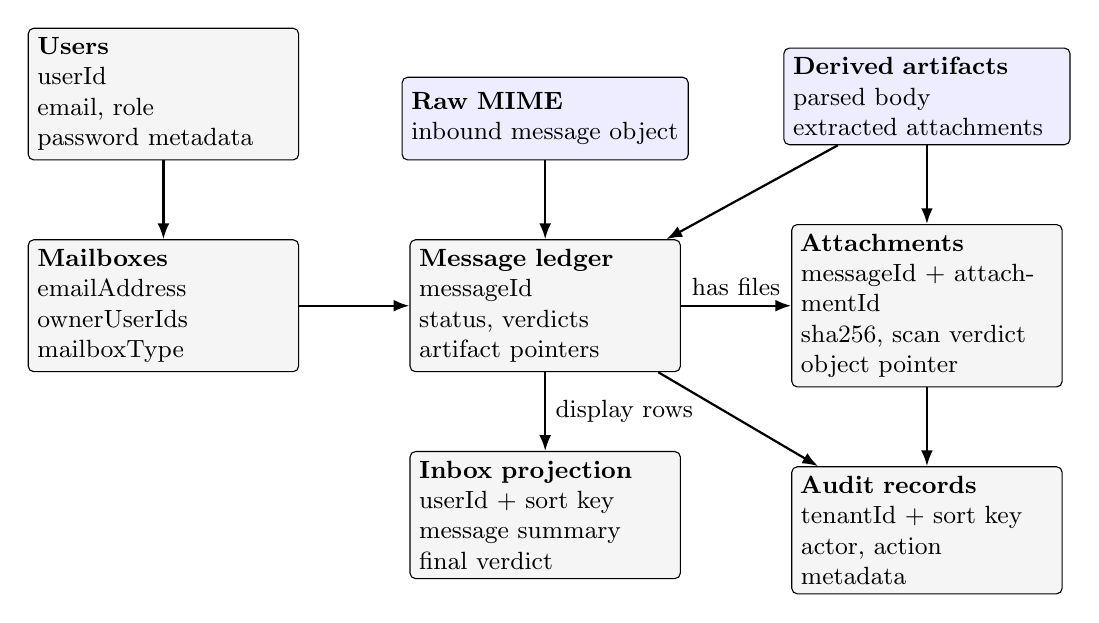
\begin{tikzpicture}[
  font=\small,
  entity/.style={draw, rounded corners=2pt, align=left, text width=3.2cm, minimum height=1.25cm, fill=gray!8},
  artifact/.style={draw, rounded corners=2pt, align=left, text width=3.4cm, minimum height=1.05cm, fill=blue!7},
  arrow/.style={-{Latex[length=2mm]}, thick},
  node distance=1.0cm and 1.4cm
]
\node[entity] (messages) {\textbf{Message ledger}\\messageId\\status, verdicts\\artifact pointers};
\node[entity, left=of messages] (mailboxes) {\textbf{Mailboxes}\\emailAddress\\ownerUserIds\\mailboxType};
\node[entity, above=of mailboxes] (users) {\textbf{Users}\\userId\\email, role\\password metadata};
\node[entity, right=of messages] (attachments) {\textbf{Attachments}\\messageId + attachmentId\\sha256, scan verdict\\object pointer};
\node[entity, below=of messages] (inbox) {\textbf{Inbox projection}\\userId + sort key\\message summary\\final verdict};
\node[entity, below=of attachments] (audit) {\textbf{Audit records}\\tenantId + sort key\\actor, action\\metadata};

\node[artifact, above=of messages] (raw) {\textbf{Raw MIME}\\inbound message object};
\node[artifact, above=of attachments] (parsed) {\textbf{Derived artifacts}\\parsed body\\extracted attachments};

\draw[arrow] (users) -- (mailboxes);
\draw[arrow] (mailboxes) -- (messages);
\draw[arrow] (messages) -- node[above]{has files} (attachments);
\draw[arrow] (messages) -- node[right]{display rows} (inbox);
\draw[arrow] (raw) -- (messages);
\draw[arrow] (parsed) -- (messages);
\draw[arrow] (parsed) -- (attachments);
\draw[arrow] (messages) -- (audit);
\draw[arrow] (attachments) -- (audit);
\end{tikzpicture}
}
\caption{Main persisted entities and artifact pointers used by the analysis workflow.}
\label{fig:data-model}
\end{figure}

Figure~\ref{fig:data-model} summarizes the stored entities. The message ledger is the central record. Inbox projections are optimized for user-specific inbox queries. Attachment records hold per-file metadata, storage pointers, hashes, and scan results. Users and mailboxes support authentication and recipient ownership. Audit records store security-relevant actions.

\begin{table}[!htbp]
\papertablecaption{tab:artifacts}{Persisted records and artifacts}
\centering
\footnotesize
\begin{tabular}{|>{\raggedright\arraybackslash}p{0.23\textwidth}|>{\raggedright\arraybackslash}p{0.27\textwidth}|>{\raggedright\arraybackslash}p{0.40\textwidth}|}
\hline
\textbf{Store} & \textbf{Key or identifier} & \textbf{Purpose} \\
\hline
S3 raw email & Inbound message object key & Preserves the original MIME message for inspection and reprocessing. \\
\hline
S3 parsed body & Message-scoped parsed artifact key & Stores parsed headers, summary, plain text, HTML, and attachment summaries. \\
\hline
S3 attachments & Message-scoped attachment object keys & Stores extracted attachment bytes separately from workflow payloads. \\
\hline
DynamoDB message ledger & \texttt{messageId} & Central state for status, ownership, raw/artifact pointers, and verdicts. \\
\hline
DynamoDB inbox projection & \texttt{userId}, time-sort key & User-specific query rows with display status and verdicts. \\
\hline
DynamoDB attachment records & \texttt{messageId}, \texttt{attachmentId} & Per-file metadata, SHA-256, scanner status, verdict, and signature. \\
\hline
DynamoDB audit records & \texttt{tenantId}, time-sort key & Records security-relevant actions such as login, view, reprocess, and download. \\
\hline
\end{tabular}
\end{table}


The split between S3 artifacts and DynamoDB records is intentional. Raw MIME messages, parsed bodies, and attachment bytes are large or semi-structured objects and belong in object storage. DynamoDB stores compact state, ownership, verdicts, and pointers. Step Functions passes identifiers and S3 locations rather than embedding whole email bodies or files in workflow payloads. This keeps each stage focused and makes reprocessing possible from the raw pointer.

\section{Classification, Attachment Scanning, and Verdict Aggregation}

The detection layer has three parts: phishing text classification, attachment scanning, and final verdict aggregation. The project does not assume that a single detector is sufficient. Each detector contributes evidence that is stored and then simplified into a message-level verdict for the dashboard.

\subsection{Text Classification}

The ML inference stage loads a packaged phishing model and a packaged TF-IDF vectorizer. The training code defines a TF-IDF vectorizer with 15,000 maximum features, word unigrams and bigrams, minimum document frequency of 10, and English stop-word removal. It compares logistic regression, multinomial Naive Bayes, random forest, and a linear SGD classifier. The training script selects the best model by validation accuracy, while the checked-in evaluation plot also reports precision, recall, and F1. The packaged classifier follows the SGD path with modified Huber loss and balanced class weights.

The text normalization step lowercases input, replaces URL-like tokens, removes selected mail headers and corpus-specific tokens, replaces digits, removes most punctuation except common email characters, and collapses whitespace. The cleaned subject and body text are then transformed into TF-IDF features. scikit-learn is the underlying ML library; its JMLR paper describes it as a Python module covering supervised and unsupervised learning algorithms with a consistent API \cite{pedregosa2011scikit}. A compact formulation of the representation is:

\begin{equation}
x_{d,t} = \mathrm{tf}(t,d) \cdot \log\left(\frac{1 + N}{1 + \mathrm{df}(t)}\right),
\label{eq:tfidf}
\end{equation}

where \(x_{d,t}\) is the feature value for term \(t\) in document \(d\), \(N\) is the number of training documents, and \(\mathrm{df}(t)\) is the number of documents containing term \(t\). The exact smoothing and normalization are delegated to the saved vectorizer parameters.

The inference output is an ML object with verdict, category, score stored in the \texttt{confidence} field, model version, model source, and feature version. Prediction value \(1\) is interpreted as \texttt{PHISHING}; other predictions become \texttt{LOW\_RISK}. The choice of a TF-IDF linear model is conservative but defensible for a workflow stage because it is fast, explainable at the feature level, and supported by strong baselines in phishing email literature \cite{fette2007learning,altawil2024comparative}.

\subsection{Attachment Scanning}

The attachment scanner uses records produced by the parser. For each attachment, it reads the object, computes SHA-256, invokes \texttt{clamscan}, and maps the scanner result into \texttt{SAFE}, \texttt{UNSAFE}, \texttt{SCAN\_ERROR}, or \texttt{TIMEOUT}. The scanner also stores any ClamAV signature string returned by the command. The production engineering track includes a managed signature update lifecycle so scanner definitions remain fresh over time.

The project deliberately stores attachment scan data per file rather than only at the message level. This lets the dashboard show which file triggered an unsafe verdict, the filename, content type, size, SHA-256 hash, signature, scan status, and download action. It also allows the aggregate stage to recompute message-level virus state from child records.

\subsection{Final Verdict Rules}

Final verdict aggregation is intentionally simple. Let \(m\) be the ML verdict and \(v\) be the aggregate attachment verdict. The current implementation can be written as:

\begin{equation}
F(m,v)=
\begin{cases}
\texttt{UNSAFE}, & m=\texttt{PHISHING} \lor v=\texttt{UNSAFE},\\
\texttt{SUSPICIOUS}, & m\in\{\texttt{ERROR},\texttt{PENDING}\} \lor v=\texttt{PARTIAL},\\
\texttt{SAFE}, & \text{otherwise.}
\end{cases}
\label{eq:verdict}
\end{equation}

The aggregate virus verdict is \texttt{SAFE} when there are no attachments or all attachments are safe, \texttt{UNSAFE} when at least one attachment is unsafe, and \texttt{PARTIAL} when any scan remains pending or ends in an error-like state. This rule set is conservative: unavailable detector data does not become a clean result.

\section{Dashboard and Review Workflow}

The backend is a FastAPI application with authentication routes, message routes, admin routes, audit logic, and a Lambda-compatible handler. The frontend is a React application. The important security boundary is server-side authorization: frontend navigation changes the user experience, but the API decides which records a caller may read or modify.

Authentication currently uses application-managed HS256 JWTs backed by user records. Password verification uses PBKDF2-SHA256 with per-user salt and iteration metadata stored in the user record. Tokens carry subject, email, role, tenant, and expiry claims. The planned AWS identity track is Cognito migration so user and token management can be delegated to a managed identity service.

Normal users can list and view only messages mapped to their user identifier through inbox projections and owner identifiers. Administrators can access broader review endpoints. Message detail, indicators, timeline, attachment list, and attachment download repeat the same ownership-or-admin check. This repetition matters because direct API calls should not bypass frontend navigation.

The dashboard exposes several user-visible workflows. The inbox screen provides search, status filters, verdict filters, attachment filters, sorting, pagination, and compact message rows. The message detail screen loads the message, attachments, indicators, and workflow timeline. It displays threat summary, verdict cards, email body views, metadata, ML analysis, workflow timeline, threat evidence, URLs and domains, hashes, and attachment cards. Risky attachment downloads require explicit acknowledgement before the browser downloads the file. The API also logs safe and risky download actions.

Administrators receive additional review screens. The admin dashboard shows security totals, verdict counts, top senders, mailbox activity, trends, recent messages, audit events, users, and mailbox mappings. The admin message review page supports filtering and pagination over all messages. The audit log page supports filtering by action, actor, role, and message identifier. The reprocess endpoint can start a new workflow execution for a message with an available raw artifact pointer.

\section{Evaluation Results}

The strongest quantitative evidence in the repository is the set of checked-in ML evaluation artifacts. They report a comparison between logistic regression, multinomial Naive Bayes, random forest, and the SGD-based classifier used by inference. The classifier comparison plot shows the SGD model as the best of the four evaluated models, with accuracy, precision, recall, and F1 all near 0.983. Logistic regression is close behind, while Naive Bayes and random forest trail on the same metrics. These values are treated as training-bundle evidence for the packaged model, not as claims about live organizational traffic.

\begin{figure}[!htbp]
\centering
\resizebox{0.96\textwidth}{!}{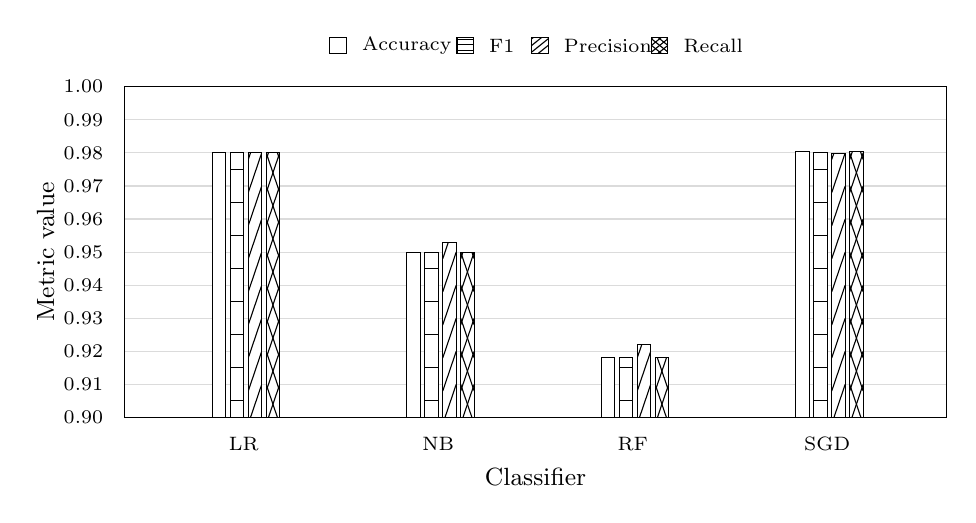
\begin{tikzpicture}[font=\scriptsize,x=0.95cm,y=4.2cm]
  \def\xmin{0}
  \def\xmax{11.0}
  \def\barw{0.18}

  \foreach \yt/\ylab in {
    0.0/0.90,
    0.1/0.91,
    0.2/0.92,
    0.3/0.93,
    0.4/0.94,
    0.5/0.95,
    0.6/0.96,
    0.7/0.97,
    0.8/0.98,
    0.9/0.99,
    1.0/1.00
  }{
    \draw[gray!28] (\xmin,\yt) -- (\xmax,\yt);
    \node[anchor=east] at (-0.15,\yt) {\ylab};
  }
  \draw[black] (\xmin,0) -- (\xmax,0) -- (\xmax,1.0) -- (\xmin,1.0) -- cycle;

  \node[font=\small, rotate=90] at (-1.05,0.5) {Metric value};
  \node[font=\small] at (5.5,-0.18) {Classifier};

  \foreach \x/\name/\acc/\fone/\prec/\rec in {
    1.6/LR/0.800/0.800/0.800/0.800,
    4.2/NB/0.500/0.500/0.530/0.500,
    6.8/RF/0.180/0.180/0.220/0.180,
    9.4/SGD/0.803/0.801/0.798/0.805
  }{
    \node[anchor=north] at (\x, -0.03) {\name};
    \draw[draw=black, fill=white] (\x-0.42,0) rectangle ++(\barw,\acc);
    \draw[draw=black, fill=white] (\x-0.18,0) rectangle ++(\barw,\fone);
    \begin{scope}
      \clip (\x-0.18,0) rectangle ++(\barw,\fone);
      \foreach \yy in {0.05,0.15,0.25,0.35,0.45,0.55,0.65,0.75,0.85}
        \draw[thin] (\x-0.18,\yy) -- ++(\barw,0);
    \end{scope}
    \draw[draw=black, fill=white] (\x+0.06,0) rectangle ++(\barw,\prec);
    \begin{scope}
      \clip (\x+0.06,0) rectangle ++(\barw,\prec);
      \foreach \yy in {-0.12,-0.02,0.08,0.18,0.28,0.38,0.48,0.58,0.68,0.78,0.88}
        \draw[thin] (\x+0.06,\yy) -- ++(\barw,0.12);
    \end{scope}
    \draw[draw=black, fill=white] (\x+0.30,0) rectangle ++(\barw,\rec);
    \begin{scope}
      \clip (\x+0.30,0) rectangle ++(\barw,\rec);
      \foreach \yy in {-0.12,-0.02,0.08,0.18,0.28,0.38,0.48,0.58,0.68,0.78,0.88} {
        \draw[thin] (\x+0.30,\yy) -- ++(\barw,0.12);
        \draw[thin] (\x+0.30,\yy+0.12) -- ++(\barw,-0.12);
      }
    \end{scope}
  }

  \draw[draw=black, fill=white] (2.75,1.10) rectangle ++(0.22,0.05);
  \node[anchor=west] at (3.05,1.125) {Accuracy};
  \draw[draw=black, fill=white] (4.45,1.10) rectangle ++(0.22,0.05);
  \begin{scope}
    \clip (4.45,1.10) rectangle ++(0.22,0.05);
    \foreach \yy in {1.110,1.127,1.144} \draw[thin] (4.45,\yy) -- ++(0.22,0);
  \end{scope}
  \node[anchor=west] at (4.75,1.125) {F1};
  \draw[draw=black, fill=white] (5.45,1.10) rectangle ++(0.22,0.05);
  \begin{scope}
    \clip (5.45,1.10) rectangle ++(0.22,0.05);
    \foreach \yy in {1.085,1.105,1.125,1.145} \draw[thin] (5.45,\yy) -- ++(0.22,0.04);
  \end{scope}
  \node[anchor=west] at (5.75,1.125) {Precision};
  \draw[draw=black, fill=white] (7.05,1.10) rectangle ++(0.22,0.05);
  \begin{scope}
    \clip (7.05,1.10) rectangle ++(0.22,0.05);
    \foreach \yy in {1.085,1.105,1.125,1.145} {
      \draw[thin] (7.05,\yy) -- ++(0.22,0.04);
      \draw[thin] (7.05,\yy+0.04) -- ++(0.22,-0.04);
    }
  \end{scope}
  \node[anchor=west] at (7.35,1.125) {Recall};
\end{tikzpicture}
}
\caption{Classifier comparison reconstructed from the checked-in ML evaluation plot.}
\label{fig:ml-comparison}
\end{figure}

The internal validation confusion matrix reports 7,748 true negatives, 158 false positives, 152 false negatives, and 7,649 true positives. Computed from those visible counts, internal validation accuracy is 0.9803. The class-1 precision, recall, and F1 are approximately 0.9798, 0.9805, and 0.9801. The Nazario split matrix reports 17 false negatives and 296 true positives, corresponding to 0.9457 class-1 recall on that artifact.

\begin{table}[!htbp]
\papertablecaption{tab:ml-results}{ML evaluation values reported by checked-in artifacts}
\centering
\footnotesize
\begin{tabular}{|>{\raggedright\arraybackslash}p{0.29\textwidth}|>{\raggedright\arraybackslash}p{0.31\textwidth}|>{\raggedright\arraybackslash}p{0.30\textwidth}|}
\hline
\textbf{Artifact} & \textbf{Reported or derived value} & \textbf{Interpretation} \\
\hline
Internal validation confusion matrix & TN 7748, FP 158, FN 152, TP 7649 & Accuracy 0.9803; phishing precision 0.9798, recall 0.9805, F1 0.9801. \\
\hline
Classifier comparison & SGD model near 0.983 on accuracy, precision, recall, and F1 & Best model among the four plotted classifiers. \\
\hline
Nazario split matrix & FN 17, TP 296 & Class-1 recall 0.9457. \\
\hline
Comparison dataset plot & Nazario 0.946, Nigerian\_Fraud 0.991 & Training-bundle evidence for classifier behavior on the named plotted sources. \\
\hline
Dataset distribution & CEAS\_08 49.8\%, Enron 37.7\%, SpamAssassin 7.4\%, Ling 3.6\%, Nazario 1.6\% & Shows a mixed corpus rather than a single-source training set. \\
\hline
\end{tabular}
\end{table}


The dataset distribution plot reports CEAS\_08 as the largest source at 49.8\%, followed by Enron at 37.7\%, SpamAssassin at 7.4\%, Ling at 3.6\%, and Nazario at 1.6\%. Enron is a well-known email corpus introduced for email classification research \cite{klimt2004enron}; the other named sources are represented in curated phishing-email and spam-corpus distributions \cite{champa2024curated,spamassassin_corpus,fraudulent_email_corpus}. The comparison plot labels Nazario split accuracy as 0.946 and Nigerian\_Fraud accuracy as 0.991. ROC plots label both train and validation AUC as 1.00, while the log-loss plots show low training and validation loss values. These results are best read as artifacts of the current training bundle and as support for using the packaged classifier inside the triage workflow.

Implementation validation is broader than the ML graphs. Unit tests cover parser behavior for body extraction, attachment extraction, artifact writing, and failure marking. API tests cover authorized and unauthorized attachment download, missing attachments, paginated listing, and audit-log failure handling. Ledger tests cover initial row creation and duplicate-message behavior. Together, these checks support the claim that the paper's main stages are not merely diagrammed; they are represented by executable components.

\section{Limitations and Future Work}

The first limitation is detector scope. The phishing classifier scores text, and ClamAV scans extracted files. Sender reputation, URL reputation, sandbox detonation, attachment content disarm, DKIM/SPF/DMARC policy reasoning, and organization-specific allow/block logic are outside the current detector set. The architecture leaves room for these signals because verdict aggregation already combines independent evidence streams.

The second limitation is operational policy. Attachment handling can be expanded with explicit size limits, archive-depth rules, retention policy, quarantine policy, and reviewer escalation rules. Raw HTML rendering must remain sanitized or isolated, and risky-download controls should be paired with organizational policy rather than treated as a complete safety boundary.

The third limitation is identity and scanner operations. The authentication layer is moving toward Cognito so identity, token handling, and user lifecycle can be managed as AWS services. The ClamAV stage needs a production signature-update lifecycle so scan definitions stay current across function/container lifetimes.

Future work follows from these limits. The workflow can add URL and domain reputation checks, header-authentication scoring, richer indicator extraction, and separate aggregation weights for phishing and malware evidence. The dashboard can add analyst notes, case assignment, exportable reports, and retention controls. The ML workflow can add threshold calibration and model cards so classifier changes are reviewable over time.

\section{Conclusions}

Cloud Email Analyzer presents an AWS-oriented architecture for turning inbound email into reviewable security evidence. The project receives MIME messages, stores original content, normalizes ingestion through \texttt{MailReceived}, resolves recipient ownership, parses body and attachments, runs text classification, scans files, aggregates verdicts, and exposes the results through an authenticated dashboard with user and administrator views.

The strongest idea is not a single detector. It is the separation between ingress, analysis, storage, verdict aggregation, and review. Raw artifacts remain available, parsed artifacts are stored separately, detector outputs are visible, attachment evidence is preserved per file, and user actions are audited. That gives the system a credible path from incoming mail to accountable security triage, while leaving space for stronger detectors, managed identity, and operational hardening.

\begingroup
\raggedright
\bibliographystyle{ieeetr}
\bibliography{references}
\endgroup

\end{document}
